\documentclass[12pt,letterpaper]{article}

\pdfoutput=1

\usepackage[OT1]{fontenc}
\usepackage[colorlinks,citecolor=blue,urlcolor=blue]{hyperref}
\usepackage[pdftex]{graphicx}
\usepackage{subfig}
\usepackage{fullpage}
\usepackage{palatino}
\usepackage{mathpazo}
\usepackage{amsmath}
\usepackage{amsfonts}
\usepackage{amsthm}
\usepackage{amssymb}
\usepackage{color}
\usepackage{todonotes}
\usepackage{listings}
\usepackage{framed}
\usepackage{common}
\usepackage{graphicx}
\usepackage[mmddyyyy,hhmmss]{datetime}
\newcommand{\Bern}{\operatorname{Bern}}
\newcommand{\argmax}{\operatorname{argmax}}
\newcommand{\norm}[1]{\left\lVert#1\right\rVert}
\newcommand{\BR}{\mathbb R}

\newtheorem{exercise}{Exercise}

\newboolean{solutionCopy}
\setboolean{solutionCopy}{true} 

\ifthenelse{\boolean{solutionCopy}}{
  \includeversion{solution}
}{
  \excludeversion{solution}
}

\newenvironment{exercisesolution}
  {\begin{proof}[Solution]}
  {\end{proof}}

\begin{document}

\ifthenelse{\boolean{solutionCopy}}{
\begin{center}
{\LARGE CS 181 Spring 2018 Section 8\\
Mixture Modeling and EM}
\end{center}
}{
  \begin{center}
{\LARGE CS 181 Spring 2018 Section 8}\\
Topic Modeling and EM
\end{center}
}

\section{Graphical Models}
We can represent a large class of probabilistic models within the framework of \emph{directed graphical models}. A directed graphical model is a visual representation that shows the conditional relationships between parameters, latent variables, and observed variables, and provides a language for factorizing a joint distribution. 

\smallskip

\begin{exercise}
Use the following graphical model to factorize the joint distribution $p(\boldx, \boldy | \theta, \bpi_1, \bpi_2)$. Which of the models we have studied in this class does this graphical model represent? \\
\begin{center}
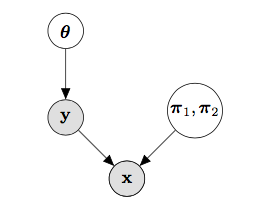
\includegraphics[width=7cm]{graphical_model}
\end{center}
\end{exercise}
\begin{exercisesolution}
%$p(\boldx, \boldy | \theta, \bpi_1, \bpi_2) = p(\boldy | \theta)p(\boldx | \boldy, \bpi_1, \bpi_2) $. This is the graphical representation of the Naive Bayes algorithm we saw earlier in the class.
\newpage

\end{exercisesolution}

\section{Mixture Models}

A \emph{mixture model} is a type of probabilistic
model for unsupervised learning. The basic idea is the following:
we assume that our data is generated by 
first sampling a category from some predefined
set, and then sampling an observation within
that category. That is, we sample a latent
variable $\boldz$ according to a categorical
distribution $p(\boldz = C_k; \btheta) = \theta_k$, and
then sample an observation $\boldx$ from
some distribution $p(\boldx | \boldz)$.

\smallskip

Mixture models are very useful for modeling
\emph{latent variables}, i.e., variables that aren't 
directly observed at training time, but are
still part of the data generation process. For 
example, we can cluster data by fitting a mixture
model, and then determining the most likely
latent class for each data point. Unfortunately,
training mixture models cannot be done 
simply in closed form. Instead we need to use
a form of approximate maximum-likelihood estimation
called \emph{expectation maximization}.



\section{Expectation Maximization}
Expectation maximization is a general technique for maximum-likelihood estimation used primarily for models with latent variables. While we talk primarily here about mixture models, EM is often used for a variety of other models.

\smallskip 

Consider a generative mixture model consisting of a latent variable $\mbz$ from a distribution $p(\mbz; \boldw)$ and an observed variable $\boldx$, such that we draw $\boldx$ from a distribution $p(\boldx | \mbz; \boldw)$ for some vector of parameters $\boldw$. 

\smallskip

We have 2 goals: first, to compute the MLE for $\boldw$, i.e. the value of $\boldw$ that maximizes $p(\boldx; \boldw)$, and second, to estimate the latent variable $\mbz$ corresponding to a particular $\boldx$, which in this case means maximize the distribution $p(\mbz | \boldx; \boldw)$. The latter goal is easy once we have an estimate of the MLE for $\btheta$, because we can apply Bayes rule:
\begin{align}p(\mbz | \boldx; \boldw) \propto p(\boldx | \mbz; \boldw)p(\mbz; \boldw)\end{align}
So all we need to do is build a model for the generative process ($p(\boldx | \mbz; \boldw)$ and $p(\mbz; \boldw)$), and determine out how to calculate the MLE.

\subsection{Why EM?}
Unfortunately calculating the MLE is often computationally intractable, because the log-likelihood is:
\begin{align}
    \log p(\boldx; \boldw) = \log \sum_{\boldz \in Z} p(\boldx, \mbz; \boldw)
\end{align}
We know the form of the model $p(\boldx, \mbz; \boldw)$, but in general we don't know the likelihood $p(\boldx; \boldw)$ in closed form. There is no closed form expression for the MLE because it is the log of a sum of expressions, which makes simplifying difficult. Note that we've assumed that our latent variable $\boldz$ takes on values in a discrete space $Z$ (below, that space will be a set of class labels or clusters, and thus $Z = \{C_k\}_{k=1}^c$, and $\boldz$ is one-hot)--- things get even more difficult in the continuous case (the sum becomes an integral, etc.).

\subsection{Algorithm}
Since finding the MLE directly is difficult, we will use an approximate iterative approach. This takes the following form: we approximate the MLE, approximate the distribution of the latent variables $\mbz$, and repeat until the approximation is very good. This makes the problem simpler, since we usually have good ways to find the MLE given the value of the $\mbz$, and to find the distribution of $\mbz$ given the MLE. In particular, if we know the value of $\boldw$, then the distribution of $\mbz$ is $p(\mbz | \boldx; \boldw)$. Additionally if we know the distribution of $\mbz$, then the expected complete data log-likelihood is tractable, since we are calculating:
\begin{align}
\E_{\boldz | \boldx ; \boldw}\left[ \sum_{i = 1}^n\log p(\boldx_i, \mbz_i; \boldw)\right]
&= \E_{\boldz | \boldx ; \boldw}\left[\sum_{i = 1}^n\left(\log p(\boldx_i | \mbz_i; \boldw) + \log p(\mbz_i; \boldw)\right)\right] \\
&= \sum_{\boldz \in \mcZ} p(\boldz | \boldx ; \boldw) \left[\sum_{i = 1}^n (\log p(\boldx_i | \boldz_i;\boldw) + \log p(\boldz_i ; \boldw)) \right] \\
&= \sum_{\boldz \in \mcZ} q(\boldz) \left[\sum_{i = 1}^n (\log p(\boldx_i | \boldz_i ; \boldw) + \log p(\boldz_i ; \boldw)) \right]
\end{align}
where $p(\boldz | \boldx ; \boldw) = q(\boldz)$. So the steps of the algorithm are:
\begin{enumerate}
	\item Initialize a $\boldw^{(0)}$ randomly (what are we trying to avoid in this initialization?).
	\item Calculate the distribution $\boldq$ over $\mbz$:
	\begin{align} q_{i,k} = p(\mbz_i = C_k | \boldx_i; \boldw^{(i)}) \propto p(\boldx_i | \mbz_i; \boldw^{(i)})p(\mbz_i; \boldw^{(i)})\end{align}
	\item Choose the value of $\boldw^{(i+1)}$ that maximizes the expected complete data log likelihood (where the expectation is over the distribution calculated above):
	\begin{align}\boldw^{(i+1)} = \underset{\boldw}\argmax\: \E_{\mathbf{q}}\left[\log p(\boldx, \mbz; \boldw)\right]
	\end{align}
	\item Go back to step 2 until the log likelihood estimate converges.
\end{enumerate}

\subsection{Example 1 - Coins}

Consider a setup where we have 2 biased coins. We generate data by picking between the two coins with another biased coin, and then flip the chosen coin to generate a new data point $x_i$. We wish to do inference on the parameters of the coins, but the only data we're given is the outcomes of the flips.

Here, we have a very clear choice of $\boldz_i$: a value that indicates whether the $i$th coin flip was from the first or second coins. To keep parity with the lecture, which essentially uses the same model for the mixture of multinomials, we'll let the variable $\boldz_i$ be a one-hot vector (of size 2) indicating which coin it came from. Also, we'll denote the vector of probabilities for the coin used to choose between coins as $\btheta \in \BR^2$, where $\theta_1$ is the probability we'll pick the first coin, and $\theta_2$ the second. Finally, we'll use $\bpi_1, \bpi_2 \in \BR^{2}$  to denote the biases for each coin, where $\bpi_1$ is the vector of probabilities for coin 1, etc. This is exactly the same setup as in class for a mixture of multinomials except we only have two multinomials here (coins 1 and 2) and they have 2 outcomes (heads or tails). We let $\boldw := \{\btheta, \bpi\}$.



\begin{exercise}
Draw a graphical model that represents this generative process.\\\\
\end{exercise}

\begin{exercisesolution}
%\begin{center}
%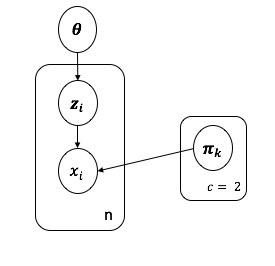
\includegraphics[width=5cm]{coins_plate}
%\end{center}
\end{exercisesolution}
\vspace{3cm} 

\noindent First we note that we can calculate $\boldq_i$ from $\boldw^{(i)}$ by writing:
	\begin{align}
		\boldq_i &= \begin{bmatrix}p(\boldz_i = C_1 | \boldx_i; \boldw^{(i)}) \\ p(\boldz_i = C_2 | \boldx_i; \boldw^{(i)})\end{bmatrix} \\
		    &\propto \begin{bmatrix}p(\boldx_i | \boldz_i = C_1; \boldw^{(i)})p(\boldz_i = C_1; \boldw^{(i)}) \\ p(\boldx_i | \boldz_i = C_2; \boldw^{(i)})p(\boldz_i = C_2; \boldw^{(i)})\end{bmatrix} \\
			&\propto \begin{bmatrix}(\pi_{11})^{x_1}(\pi_{12})^{x_2}\theta_1\\ (\pi_{21})^{x_1}(\pi_{22})^{x_2}\theta_2\end{bmatrix}
	\end{align}
\noindent We also have the data log-likelihood as
	\begin{align}
	\log p(\boldx_i, \boldz_i; \boldw) &= \log p(\boldx_i | \boldz; \boldw)p(\boldz; \boldw)\\
	    &= \log \prod_{k = 1}^{c = 2}\left(\theta_k\prod_{j = 1}^{2}\pi_{kj}^{x_{ij}}\right)^{z_{ik}}\\
	    &= z_{i1}\left(\log\theta_1 + x_{i1}\log \pi_{11} + x_{i2}\log \pi_{12}\right) \\
	    &+ z_{i2}\left(\log\theta_2 + x_{i1}\log \pi_{21} + x_{i2}\log \pi_{22}\right) \\
    \log p(\boldx, \boldz; \boldw) &= \sum_{i = 1}^n \log p(\boldx_i, \boldz_i; \boldw)
	\end{align}
Finally, if we have an estimate for $\boldq$, we also have
	\begin{align}
		\mcL_{c} &= \E_{\boldz | \boldx ; \boldw}\left[\sum_{i = 1}^n \log p(\boldx_i, \mbz_i; \boldw)\right]\\
		&= \E_{\boldz | \boldx ; \boldw} \left[\sum_{i=1}^n\log p(\boldz_i ; \boldw) + \log p(\boldx_i | \boldz_i ; \boldw) \right] \\
		&= \sum_{i = 1}^n \E_{\boldz | \boldx ; \boldw} \left[ \log p(\boldz_i ; \boldw) + \log p(\boldx_i | \boldz_i ; \boldw)\right]\\
		&= \sum_{i = 1}^n \sum_{k = 1}^c q_{ik}\left(\log \theta_k + \sum_{j = 1}^2 x_{ij} \log \pi_{kj}\right) \\
		&= \sum_{i = 1}^n q_{i1}\left(\log\theta_1 + x_{i1}\log \pi_{11} + x_{i2}\log \pi_{12}\right) + q_{i2}\left(\log\theta_2 + x_{i1}\log \pi_{21} + x_{i2}\log \pi_{22}\right)
	\end{align}
	since $\boldq$ is just a pair of probabilities for each example.
This gives us everything we need to use expectation-maximization.
Let's walk through the steps:
\begin{enumerate}
	\item Initialize $\boldw^{(0)}$ randomly.
	\item Use $\boldw^{(i)}$ to calculate the vector of probabilities $\boldq_i$ for the distribution of each $\boldz_i$ (eqs. 8-10).
	\item Calculate the approximate expected likelihood using $\boldq_i$ and $\boldw^{(i)}$ (eqs. 11-15). This step is not strictly necessary for calculating updates, but can be helpful for a variety of purposes, including debugging and testing convergence. Note that we need \emph{both} $\boldq$ and $\boldw^{(i)}$ to get a value here.
	\item Use $\boldq$ to calculate an updated set of parameters $\boldw^{(i+1)}$ by maximizing the expected likelihood as a function of $\boldw$ (eqs. 16-20). Note that here we do \emph{not} use $\boldw^{(i)}$. 
	
	\smallskip
	
	During optimization we need to enforce that $\sum_k \theta_k = 1$ and that $\sum_j \pi_{kj} = 1$, so that the distributions parameterized by $\btheta$ and $\bpi$ valid. In general we want to use Langrange multipliers, but in this case we can substitute $\theta_2 = 1 - \theta_1$ and $\pi_{k2} = 1 - \pi_{k1}$:
	\begin{align}
	    \mcL_c = \sum_{i = 1}^n \enspace&q_{i1}\left(\log\theta_1 + x_{i1}\log \pi_{11} + x_{i2}\log (1 - \pi_{11})\right) \\
	    + &q_{i2}\left(\log(1 - \theta_1) + x_{i1}\log \pi_{21} + x_{i2}\log(1 - \pi_{21})\right)
	\end{align}
	And then optimize w.r.t. $\theta_1, \pi_{11}, \pi_{21}$:
	\begin{align}
		\frac{\partial \mcL_c}{\partial \theta_1} &= \sum_{i = 1}^n \left(\frac{q_{i1}}{\theta_1} - \frac{q_{i2}}{1 - \theta_1}\right) = 0 \\
		\frac{\partial \mcL_c}{\partial \pi_{11}} &= \sum_{i = 1}^n q_{i1}\left(\frac{x_{i1}}{\pi_{11}} - \frac{x_{i2}}{1 - \pi_{11}}\right) = 0 \\
		\frac{\partial \mcL_c}{\partial \pi_{21}} &= \sum_{i = 1}^n q_{i2}\left(\frac{x_{i1}}{\pi_{21}} - \frac{x_{i2}}{1 - \pi_{21}}\right) = 0
	\end{align}
	From here we can solve for the optimal value of $\boldw$ (i.e. $\theta_1, \pi_{11}, \pi_{22}$), and set $\boldw^{(i+1)} = \argmax_{\boldw} \E_{\boldz | \boldx ; \boldw} \mcL_c$.
\end{enumerate}
\emph{Note}: Above we show the derivation of all steps of the algorithm, but in practice $\boldw^{(i+1)}$ has a closed form, so the steps of the algorithm are really just initialization, calculate the distribution $\mathbf{q}_i$ from $\boldw^{(i)}$, and then calculate $\boldw^{(i+1)}$ from $\boldq$. All the difficult work is in deriving the update equations. In more complicated models it can happen that $\boldw^{(i+1)}$ does not have a closed form, so instead we can do gradient descent to calculate the optimal value. 

\smallskip

\begin{exercise}
Derive the closed form updates for $\btheta^{(i)}, \bpi^{(i)}$ from the steps above.
\end{exercise}

\begin{exercisesolution}
%We use $t$ to refer to the $t$th step to disambiguate from indexing over the data:
%\begin{align*}
%	\theta^{(t)}_k &\leftarrow \frac{\sum_{i = 1}^n q_{ik}}{n} \\
%	\bpi^{(t)}_k &\leftarrow \frac{\sum_{i = 1}^n q_{ik}\boldx_i}{\sum_{i = 1}^n\sum_{j = 1}^m q_{ik}x_{ij}}
%\end{align*}
\end{exercisesolution}
\vspace{3cm}

Once we have an estimate for the MLE, we can use it to do prediction of hidden states for a new incoming coin flip, using step 2 from above. So, given a new coin flip, we can predict whether it can from the first or the second coin. As you can imagine, this is a terrible process, since we get a single bit of information, and in particular it is impossible to tell the difference between having one coin with high probability at 0.5 (and another picked almost never with bias = 0.1 e.g.) and two equally likely coins with biases 0.4 and 0.6. This problem is due more to the data setup rather than the method, so let's try an easier problem:\\

\begin{exercise}
Consider the following data generation process: the setup is the same as above, but instead of flipping the chosen coin once, we flip it 10 times before choosing a new coin.

\begin{enumerate}
    \item Find an appropriate choice of latent variables $\boldz_i$ and calculate the distribution of $\boldz_i$ given the data $\boldx_{i,j}$ (where $i$ iterates over the sets of 10 coin flips, and $j \in [1, 10]$) and an estimate for $\btheta$.
    \item Find the expression for the expected complete data log-likelihood
    \item Find the closed form update equations for $\btheta^{(i)}$, and compare them to the result from Exercise 1.
\end{enumerate}
\end{exercise}
\begin{exercisesolution}
%\noindent
%\begin{enumerate}
	%\item Here again we can use $\boldz_i$ to denote the 1-hot choice of the chosen coin, this time used for all 10 of the flips. The distribution of $\boldz_i$ is again proportional to the prior times the likelihood, which is:
	%$$p(\boldz_i | \boldx_i, \boldw) \propto p(\boldx_i | \boldz_i, \boldw) \cdot p(\boldz_i | \boldw) = \prod_{k = 1}^{c = 2}\left(\prod_{j = 1}^{10}\prod_{l = 1}^{2}\pi_{kl}^{x_{ijl}}\right)^{z_{ik}} \cdot \prod_{k = 1}^{c = 2}\theta_k^{z_{ik}}$$
	%where $x_{ijl}$ is the indicator variable for the $j$th coin in the $i$th set of 10 being in class $l$ (in this case, heads or tails).
	%\item The expected complete data loglikelihood is similar to the above case:
	%$$\mcL_c = \sum_{i = 1}^n \sum_{k = 1}^{c = 2} q_{ik}\left(\log \theta_k + \sum_{j = 1}^{10}\sum_{l = 1}^2 x_{ijl} \log \pi_{kj}\right)$$
	%\item In fact, $\btheta$ satisfies the same expression as before, so the update is the same:
	%$$\theta^{(t)}_k \leftarrow \frac{\sum_{i = 1}^n q_{ik}}{n}$$
	%The only thing that has changed here is the matrix $\boldq$. Remember that $q_{ik}$ is proportional to the prior probability of choosing the coin, times the likelihood. Here the likelihood term is stronger (because we see more evidence per latent variable) so we can expect this estimate to be less noisy, and thus our estimation of $\theta$ is less noisy.
%\end{enumerate}
%\smallskip
\end{exercisesolution}
\newpage

\subsection{Example 2 - Gaussian Mixture Modeling}

We covered this in class, but it's a good idea to go over some of the points in the derivation from class. Remember that the setup is that we have data $\boldx_i \in \mathbb{R}^{m}$ and a latent variable $\boldz_i$ (corresponding to the cluster that the point is drawn from) such that $\boldx \sim p(\boldx | \boldz = C_k) = \mathcal{N}(\boldx; \bmu_k, \bSigma_k)$, where $\bmu_k, \bSigma_k$ are the mean and covariance of the $k$th cluster. The choice of cluster is drawn from a categorical distribution with probabilities $\btheta \in \mathbb{R}^c$. We are able to observe the data $\boldx_i$ and want to find the cluster centers and their covariances.

Following the same format as above, the steps of EM inference applied to this problem are:
\begin{enumerate}
    \item Randomly initialize $\btheta, \{\bmu_k, \bSigma_k\}_k$.
    \item Next, calculate the new distribution of each $\mbz_i$:
        \begin{align}
            q_{ik} = p(z_i = C_k | \boldx_i) \propto \theta_k \mathcal{N}(\boldx_i; \bmu_k, \bSigma_k)
        \end{align}
    This is our new estimate of the distribution of $\mbz_i$ given the data and our estimate for $\btheta, \{\bmu_k, \bSigma_k\}_k$.
    \item Find the expected complete data log-likelihood:
    \begin{align}
         \E_{\boldZ}\left[\mcL\right] &= \E_{\boldZ}[\sum_{i = 1}^n \ln(p(\boldx_i, \boldz_i; \btheta, \{\bmu_k, \bSigma_k\}_k))] \\
         &= \sum_{i = 1}^n\sum_{k = 1}^c q_{ik} \ln \theta_k + q_{ik} \ln \mathcal{N}(\boldx_i; \bmu_k, \bSigma_k) 
    \end{align}
    and then optimize it for each of the parameters $\btheta, \{\bmu_k, \bSigma_k\}_k$. However, we need to be careful to remember constraints: since $\sum_k \theta_k = 1$, we must use Lagrange multipliers to optimize the parameters. We get the following update equations:
    \begin{align}
        \theta_k^{(i + 1)} &= \frac{\sum_{i = 1}^n q_{ik}}{n} \\
        \bmu_k^{(i + 1)} &= \frac{\sum_{i = 1}^n q_{ik}\boldx_i}{\sum_{i = 1}^n q_{ik}} \\
        \bSigma_k^{(i + 1)} &= \frac{\sum_{i = 1}^n q_{ik}(\boldx_i - \bmu_k^{(i + 1)})(\boldx_i - \bmu_k^{(i + 1)})^{\top}}{\sum_{i = 1}^n q_{ik}}
    \end{align}
\end{enumerate}

%In class we mentioned that the EM algorithm simplifies to K-means when the Gaussians are fixed to be spherical, and we take the limit of the the variance to 0. In more detail, note that when calculating $\mathbf{q}_{i}$, the vector of probabilities of cluster assignments of the $i$th point, that when $\bSigma_k = \epsilon \mathbf{I}$, then we have:
% \begin{align}
%      q_{ik} &\propto \theta_k \mathcal{N}(\boldx_i; \bmu_k, \epsilon \mathbf{I}) \\
%      \log q_{ik} &= \log \theta_k - \frac{1}{2\epsilon}\norm{\boldx_i - \bmu_k}^2
% \end{align}
% As $\epsilon \to 0$, the second term dominates, and in fact the value of $k$ with the lowest $\norm{\boldx_i - \bmu_k}^2$ (i.e. the closest cluster center to the point) gets all of the probability mass. So, in effect, the cluster assignments are hard, where $\mathbf{q}_i$ is almost a one-hot vector. What happens in the M step? Note in the updates that we don't use $\bSigma_k$, but we now know that the new values of $\bmu_k$ becomes $\sum_{q_{ik} = 1}x_i/(\sum_{q_{ik} = 1}^n q_{ik})$, which if we look closely is actually just the regular (unweighted) mean of the points assigned to cluster $k$. This is precisely the K-means algorithm.

% \subsection{Generalizations}

% Our examples in class are a limited subset of what EM is used for. First of all, the assumption that $\boldz_i$ has a distribution that we can calculate explicitly often doesn't hold, so instead of calculating the distribution, we calculate the expected complete data log likelihood directly. For example, if the complete data log-likelihood was of the form:
% \begin{align}
% \mcL &= \sum_{i = 1}^n -\frac{\boldz_i^2}{2} + f(\boldz_i)
% \end{align}
% Then we would hope that we could easily calculate the expectation of those quantities under our distribution, i.e.
% \begin{align}
%      \E_{\mbz | \boldx; \btheta}[\boldz_i^2] \text{and} \E_{\mbz | \boldx; \btheta}\left[f(\boldz_i)\right]
% \end{align}
% Depending on the scenario, we might be able to calculate the log-likelihood exactly (i.e. analytically as a function of a $\boldx_i, \btheta$), or use a method like importance sampling to estimate it. Remember that even after estimating this quantity, it remains a function of the parameters $\btheta$, and we still need to optimize it to find the next $\btheta^{(i + 1)}$.

% Let's summarize some of the practical considerations for using EM:
% \begin{enumerate}
%     {\bf Pros:} \\
%     \item  Given the right data, generative model, and choice of hidden variable, the E and M steps can sometimes be very simple and intuitive.
%     {\bf Cons:} \\
%     \item We only know that it converges to a local minimum, so we usually need random restarts (which could be a problem if the state space $\mathcal{Z} \times \bTheta$ is large).
%     \item Convergence can be slow.
%     \item There are problems where there 
% \end{enumerate}

% \section{Topic Modeling}

% Topic modeling is a form of mixture modeling commonly used in 
% analyzing text corpora. As this is a form of unsupervised learning, the goal is to extract a set of parameters
% from our data that we can use to make inferences about it.
% In particular, in topic modeling, we are interested in
% learning the topics that exist in a corpus - we will define this
% concept more formally.

% Like mixture models that we 
% study in this course, we will describe topic modeling as a
% generative model: one in which we assume our corpus is generated
% by some process. Then, we will seek to use an estimation
% technique, like EM, to determine the parameters of this model,
% and we can then interpret these parameters to understand
% the corpus.

% We begin by describing the generative process by which a document $i$ is generated. For topic modeling, similar to K-means, we have to begin by picking the number of topics, $C$, to look for. We define a topic $\bbeta_{k}$ to be a distribution over the vocabulary, so $\bbeta_{k} \in \mathbb{R}^{|\mcV|}$. For each document, we have a document-topic distribution $\btheta_i \in \mathbb{R}^C$. This is one of the parameters we will find by estimation. 

% Now, we begin sampling words. First, we sample a topic $z_{it} \sim Multinomial(\btheta_i)$. This is a latent variable representing the topic for the $t$th word in the $i$th document. Finally, we sample a word from the topic-word distribution. So, $w_{it} \sim Multinomial(\bbeta_{z_{it}})$. 

% This process is summarized in the plate diagram here:

% \includegraphics{lda}

%%% these need to be updated

\newpage
\end{document}